\chapter{Ottimizzazione}
Esaminiamo il seguente Problema di Massimo\footnote{Un problema di massimo può essere trasformato in un problema di minimo considerando la funzione -f}:
\begin{equation*}
    \begin{cases}
    \max_{\vc{x}} f(\vc{x}) \\
    con &h_i(\vc{x}) \geq 0, \forall i = 1,...,I\\
    & c_j(\vc{x}) = 0, \forall j = 1,..., J
    \end{cases}
\end{equation*}
dove:
\begin{itemize}
    \item $f$ è la Funzione Obiettivo
    \item le $h_i$ definiscono i Vincoli di Disuguaglianza
    \item gli $c_j$ definiscono i Vincoli di Uguaglianza
\end{itemize}

\section{Introduzione ai Problemi Convessi}
\subsection{Insieme Convesso}
Un insieme $C \subset \mathbb{R}^n$ si dice Convesso se e solo se $(\lambda \vc{x}_1 + (1 - \lambda)\vc{x}_2) \in C$, per ogni $\vc{x}_1, \vc{x}_2 \in C$ e $\lambda \in [0,1]$.\\ \\
\begin{center}
    (Ovvero se scelti due punti qualsiasi esiste un segmento che li congiunge senza uscire dall'insieme)
\end{center}

\subsection{Funzione Convessa}
\footnote{Una Funzione Concava si ottiene con il maggiore uguale}
Sia $C \subset \mathbb{R}^n$ un Insieme Convesso.
Allora $f : C \longrightarrow \mathbb{R}$ è Convessa se e solo se:
\begin{equation*}
    f(\lambda \vc{x}_1 + (1 - \lambda)\vc{x}_2) \leq \lambda f(\vc{x}_1) + (1 - \lambda)f(\vc{x}_2)
\end{equation*}
per ogni $\vc{x}_1, \vc{x}_2 \in C$ e $\lambda \in [0,1]$.
La Convessità diventa Stretta\footnote{Con la Concavità Stretta avremo il maggiore} con il minore.\\ \\

\begin{table}[h!]
    \centering
    \begin{tabular}{c c}
      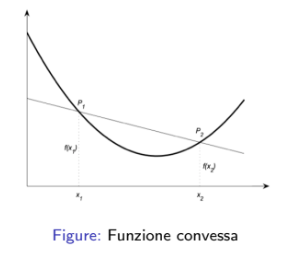
\includegraphics[]{Images/FunzioneConvessa.png}  & 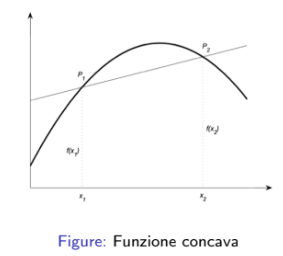
\includegraphics[]{Images/FunzioneConcava.png}
    \end{tabular}
\end{table}
\section{Condizioni al Primo Ordine}
\subsection{Funzioni Convesse Derivabili}
Sia $f : C \subset \mathbb{R}^n \longrightarrow \mathbb{R}$ differenziabile. \\ 
Allora $f$ è Convessa se e solo se:
\begin{equation*}
    f(\vc{x}_1) \geq f(\vc{x}_2) + \nabla^T f(\vc{x}_2)(\vc{x}_1 - \vc{x}_2), \quad \forall \vc{x}_1, \vc{x}_2 \in C
\end{equation*}
$f$ sarà Strettamente Convessa con il maggiore.
\begin{center}
    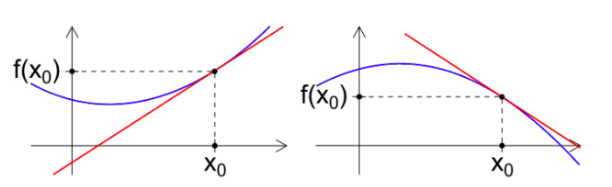
\includegraphics[width=0.8\textwidth]{Images/FunzioniDerivabiliConvesseConcave.png}
\end{center}
\subsection{Dimostrazione delle Condizioni al Primo Ordine}
Per definizione, se $f$ è Convessa\footnote{In modo analogo si dimostra per le Funzioni Concave}, allora vale:
\begin{equation*}
\begin{aligned}
    \lambda f(\vc{x}_1) + (1 - \lambda) f(\vc{x}_2) &\geq f(\lambda \vc{x}_1 + (1 - \lambda) \vc{x}_2) = \\
    &= f(\vc{x}_2 + \lambda(\vc{x}_1 - \vc{x}_2))
\end{aligned}
\end{equation*}
per ogni $\vc{x}_1, \vc{x}_2 \in C$ e $\lambda \in [0,1]$.\\ \\
Ora dividiamo entrambi i membri per $\lambda$:
\begin{equation*}
    \frac{\lambda f(\vc{x}_1) + (1 - \lambda) f(\vc{x}_2)}{\lambda} \geq \frac{f(\vc{x}_2 + \lambda(\vc{x}_1 - \vc{x}_2))}{\lambda}
\end{equation*}
\\ \\
Risolviamo rispetto a $f(\vc{x}_1)$:
\begin{equation*}
    f(\vc{x}_1) \geq f(\vc{x}_2) + \frac{f(\vc{x}_2 + \lambda(\vc{x}_1 - \vc{x}_2)) - f(\vc{x}_2)}{\lambda}
\end{equation*}
\\ \\
Facciamo tendere $\lambda \longrightarrow 0$:
\begin{equation*}
    f(\vc{x}_1) \geq f(\vc{x}_2) + \nabla^T f(\vc{x}_2)(\vc{x}_1 - \vc{x}_2)
\end{equation*}

\subsection{Sufficienza delle Condizioni al Primo Ordine}
\begin{center}
    Ogni Punto Stazionario è un Minimo Globale per Funzioni Convesse.
\end{center}
Sia $\vc{x}_2$ tale che $\nabla f(\vc{x}_2) = 0$ allora secondo la Condizione al Primo Ordine abbiamo che:
\begin{equation*}
    f(\vc{x}_1) \geq f(\vc{x}_2), \quad \vc{x}_1 \in C
\end{equation*}
\begin{center}
    Allora $\vc{x}_2$ è un punto di Minimo Globale di $f$!!
\end{center}
\subsubsection{Funzioni Note}
\begin{table}[h!]
    \centering
    \begin{tabular}{l|l}
       \textbf{Funzioni Convesse}  &  \textbf{Funzioni Concave}\\
       \hline
        \\
         Funzioni  Lineari & Funzioni  Lineari \\ \\
         $e^{ax}$ & $log(a + bx)$ \\ \\
         $x^a$, per $x>0$, $a\geq 1$ & $x^a$, per $x>0$, $0 \geq a\leq 1$ \\ \\
         $x \log(x)$ per x > 0 & $\left(\prod_{i=1}^N x_i\right)^{1/n}$ in $\mathbb{R}^n_{++}$ \\ \\
         Qualunque norma in $\mathbb{R}^n$ & $log(det(\vc{I} + \vc{X}))$, nello spazio delle $\vc{X}$ semidefinite positive
    \end{tabular}
\end{table}


\section{Proprietà delle Funzioni Convesse}
Ora elenchiamo le principali proprietà delle Funzioni Concave e Convesse.
\subsection{Inversione di Segno}
Sia $f$ una Funzione Convessa, allora $-f$ è una Funzione Concava.
\subsection{Somma Pesata di Funzioni}
Siano $f_1,...,f_N$ funzioni Convesse e siano $w_1,...,w_N$ dei coefficienti non-negativi.
Allora $\sum_{n=1}^N w_n f_n$ è convessa.
Infatti per ogni $\vc{x}_1, \vc{x}_2, \lambda \in [0,1]$ si ha:
\begin{equation*}
\begin{aligned}
        &g(\lambda \vc{x}_1 +(1 - \lambda)\vc{x}_2 ) = \sum_{n=1}^N w_n f_n (\lambda \vc{x}_1 +(1 - \lambda)\vc{x}_2 ) \leq \\
        &\leq \lambda \sum_{n=1}^N w_n f_n(\vc{x}_1) + (1 - \lambda) \sum_{n=1}^N w_n f_n(\vc{x}_2) = \\
        &= \lambda g(\vc{x}_1) +  (1 - \lambda) g(\vc{x}_2)
\end{aligned}
\end{equation*}
(Proprietà analoga per le funzioni Concave)

\subsection{Massimo Pesato di Funzioni Convesse}
Siano $f_1,...,f_N$ funzioni Convesse e siano $w_1,...,w_N$ dei coefficienti non-negativi.
Allora $\max_n(w_n f_n)$ è convessa.
Infatti per ogni $\vc{x}_1, \vc{x}_2, \lambda \in [0,1]$ si ha:
\begin{equation*}
\begin{aligned}
        &g(\lambda \vc{x}_1 +(1 - \lambda)\vc{x}_2 ) = \max_n w_n f_n (\lambda \vc{x}_1 +(1 - \lambda)\vc{x}_2 ) \leq \\
        &\leq \max_n(w_n \lambda f_n(\vc{x}_1) + (1 - \lambda)w_n f_n(\vc{x}_2)) \leq \\
        &\lambda \max_n(w_n \lambda f_n(\vc{x}_1)) + (1 - \lambda) \max_n(w_n f_n(\vc{x}_2)) = \\
        &= \lambda g(\vc{x}_1) + (1 - \lambda) g(\vc{x}_2)
\end{aligned}
\end{equation*}
(Proprietà analoghe per il Minimo Pesato di Funzioni Convesse/Concave)


\section{Problemi Convessi}
\subsection{Minimizzazione Convessa}
Siano $f$ e $\{h_k\}^K_{k=1}$ delle Funzioni Convesse definite sull'Insieme Convesso $C \subset \mathbb{R}^n$ e siano $\vc{A} \in \mathbb{R}^{m \ x \ n}, \vc{b} \in \mathbb{R}^m$.\\ 
\begin{center}
    Allora il seguente Problema di Minimo si dice Convesso.
\end{center}

\begin{equation*}
    (C_p): \begin{cases}
    \min_{\vc{x}} f(\vc{x}) \\
    con &h_k(\vc{x}) \leq 0, \forall k = 1,...,K\\
    & \vc{a}^T_l\vc{x} = \vc{b}_l, \forall l = 1,..., L
    \end{cases}
\end{equation*}
(Analoga definizione per il Massimo Concavo)

\subsection{Lagrangiano}
Dato un generico problema di minimo, in cui ipotizziamo la Funzione Obiettivo $f$ e i Vincoli $h_i, c_j$ Differenziabili:
\begin{equation*}
    \begin{cases}
    \min_{\vc{x}} f(\vc{x}) \\
    con &h_i(\vc{x}) \leq 0, \forall i = 1,...,I\\
    & c_j(\vc{x}) = 0, \forall j = 1,..., J
    \end{cases}
\end{equation*}
si deginisce Lagrangiano la seguente funzione:
\begin{equation*}
    L(\vc{x}, \vc{\lambda}, \vc{\nu}) = f(\vc{x}) + \sum_{i=1}^I \lambda_i h_i(\vc{x}) +  \sum_{j=1}^J \nu_j c_j(\vc{x}) 
\end{equation*}
dove i parametri $\vc{\lambda} \ e \ \vc{\nu}$ si dicono Moltiplicatori di Lagrange.
\subsection{Funzione Duale}
La funzione:
\begin{equation*}
    g(\vc{\lambda}, \vc{\nu}) = \min_{\vc{x}} L(\vc{x}, \vc{\lambda}, \vc{\nu})
\end{equation*}
viene detta Funzione Duale del problema.

\subsection{Duality Gap}
Se assumiamo $\lambda \geq 0$, la Funzione Duale fornisce una "stima" della soluzione:
\begin{equation*}
    \begin{aligned}
    g(\vc{\lambda}, \vc{\nu}) &= \min_{\vc{x}} L(\vc{x}, \vc{\lambda}, \vc{\nu}) = \\
    &= \min_{\vc{x}} f(\vc{x}) + \sum_{i=1}^I \lambda_i h_i(\vc{x}) +  \sum_{j=1}^J \nu_j c_j(\vc{x}) \leq \\
    &\leq  f(\vc{x}^*\footnote{\text{Corrisponde alla $\vc{x}$ corrispondente al minimo}}) + \sum_{i=1}^I \lambda_i h_i(\vc{x}^*) +  \underbrace{\sum_{j=1}^J \nu_j c_j(\vc{x}^*)}_{c_j(\vc{x}) = 0, \forall j} = \\
    &= f(\vc{x}^*) + \underbrace{\sum_{i=1}^I \lambda_i h_i(\vc{x}^*)}_{h_i(\vc{x}) \leq 0, \forall i} \leq f(\vc{x}^*)
    \end{aligned}
\end{equation*}
Quindi, dato che gli $h_i(\vc{x})$ sono negativi e i $\lambda$ sono positivi, per ottenere la stima più simile a $f(\vc{x}^*)$ si cerca di Massimizzare la Funzione Duale g, così la Funzione obbiettivo verrà sottratta a qualcosa di sempre più vicino allo 0 per ottenere l'uguaglianza nell'ultima riga qui sopra.\\ \\
Quindi definiamo Duality Gap la differenza tra la $f(\vc{x}^*)$ e la Funzione Duale:
\begin{equation*}
    f(\vc{x}^*) - g(\vc{\lambda}^*, \vc{\nu}^*)
\end{equation*}

\subsection{Dualità Forte, Dualità Debole}
Dividiamo le dualità in:
\begin{itemize}
    \item Dualità Debole se $f(\vc{x}^*) - g(\vc{\lambda}^*, \vc{\nu}^*) > 0$
    \item Dualità Forte se $f(\vc{x}^*) - g(\vc{\lambda}^*, \vc{\nu}^*) = 0$
\end{itemize}
Nel caso di Dualità Forte abbiamo che:
\begin{equation*}
\begin{aligned}
        f(\vc{x}^*) &= g(\vc{\lambda}^*, \vc{\nu}^*) = \min_{\vc{x}} L(\vc{x}, \vc{\lambda}^*, \vc{\nu}^*) = \\ 
        &= \min_{\vc{x}} f(\vc{x}) + \sum_{i=1}^I \lambda_i^* h_i(\vc{x}) +  \sum_{j=1}^J \nu_j^* c_j(\vc{x}) \leq \\
        &\leq f(\vc{x}^*) + \sum_{i=1}^I \lambda_i^* h_i(\vc{x}^*) +  \sum_{j=1}^J \nu_j^* c_j(\vc{x}^*) = \\
        &= f(\vc{x}^*) + \underbrace{\sum_{i=1}^I \lambda_i^* h_i(\vc{x}^*)}_{\text{Vuol dire che questo deve fare 0}} \leq f(\vc{x}^*)
\end{aligned}
\end{equation*}
\\ Quindi possiamo dire che:
\begin{itemize}
    \item $\sum_{i=1}^I \lambda_i^* h_i(\vc{x}^*)$ = 0
    \item $\vc{x}^*$ è un punto di Minimo del Lagrangiano in $(\vc{\lambda}^*, \vc{\nu}^*)$, ovvero:
    \begin{itemize}
        \item $f(\vc{x}^*) = \min_{\vc{x}} f(\vc{x}) + \sum_{i=1}^I \lambda_i^* h_i(\vc{x}) +  \sum_{j=1}^J \nu_j^* c_j(\vc{x})$
    \end{itemize}
    \item Quindi se voglio trovare $\vc{x}^*$ mi basta prendere la funzione qui sopra, farne il gradiente e porlo uguale a 0:
    \begin{itemize}
        \item $\nabla_{\vc{x}} L_{\vc{x}}(\vc{x}^*, \vc{\lambda}^*, \vc{\nu}^* ) = 0$
    \end{itemize}
\end{itemize}
\begin{center}
    Se il problema in questione NON è convesso, allora il gradiente del Lagrangiano posto a 0 è solo una condizione Necessaria di Ottimalità. \vspace{10pt}
    Perchè potrebbe indicare un minimo/massimo locale!!!!\\
    Mentre se il problema è Convesso, allora il Lagrangiano diventa una somma pesata di funzioni Convesse e Affini, per questo porre il suo gradiente a 0 diventa una condizione Suffuciente di Ottimalità!!!
\end{center}

\subsection{Condizioni KKT}
Le soluzioni di un generico problema di minimo sodisfano le seguenti condizioni dette KKT:
\begin{equation*}
    \begin{aligned}
    \nabla_{\vc{x}} &L_{\vc{x}}(\vc{x}, \vc{\lambda}, \vc{\nu} ) = 0 \\
    & h_i(\vc{x}) \leq 0, \forall i = 1,...,I \\
    & c_j(\vc{x}) = 0, \forall j = 1,..., J \\
    & \lambda_i(\vc{x}) \geq 0, \forall i = 1,..., I \\
    & \lambda_i h_i(\vc{x}) = 0, \forall i = 1,..., I \\
    \end{aligned}
\end{equation*}
\begin{itemize}
    \item Se il problema è Convesso:
    \begin{itemize}
        \item Le KKT sono condizioni Necessarie e Sufficienti di Ottimalità.
    \end{itemize}
    \item Se il problema NON è Convesso:
        \begin{itemize}
        \item Le KKT sono condizioni solo Necessarie Ottimalità.
    \end{itemize}
\end{itemize}


\section{Concavità Generalizzata}
\subsection{Problema Frazionale}
Siano $f, g : X \subset \mathbb{R}^n \longrightarrow \mathbb{R}$, con $g(\vc{x}) > 0$, per ogni $\vc{x} \in X$:
\begin{equation*}
    (F_p): \begin{cases}
    \max_{\vc{x}} \frac{f(\vc{x})}{g(\vc{x})} \\
    con \quad \vc{x} \in X
    \end{cases}
\end{equation*}
In questo caso il problema non è concavo, quindi le condizioni KKT sono solo Necessarie...\\ \\
Ma esiste una classe di funzioni che estende le proprietà delle funzioni concave alle funzioni fratte, ovvero le funzioni quasi concave.

\subsection{Funzioni Quasi-Concave}
Una funzione è Quasi-Concava se la restrizione della funzione ad un segmento giace al di sopra di uno dei due punti del segmento, matematicamente:
Sia $C \subset \mathbb{R}^n$ un insieme convesso, allora $f: C \longrightarrow \mathbb{R}$ è Quasi-Concava se e solo se:
\begin{equation*}
    f(\lambda \vc{x}_1 + (1 - \lambda)\vc{x}_2) \geq \min\{f(\vc{x}_1), f(\vc{x}_2) \}
\end{equation*}
per ogni $\vc{x}_1, \vc{x}_2 \in C$ e $\lambda \in [0;1]$.
\subsubsection{Funzioni Strettamente Quasi-Concave}
Partendo dalle stesse ipotesi di prima, una funzione si dice Strettamente Quasi-Concava se:
\begin{equation*}
        f(\lambda \vc{x}_1 + (1 - \lambda)\vc{x}_2) > \min\{f(\vc{x}_1), f(\vc{x}_2) \}
\end{equation*}
per ogni $\vc{x}_1, \vc{x}_2 \in C$, $\vc{x}_1 \neq \vc{x}_2$ e $\lambda \in (0;1)$.\\

\subsubsection{Esempi di funzioni Quasi-Concave}
Quindi informalmente la Quasi-Concavità pretende che la funzione cresca e poi decresca, senza ricrescere di nuovo.
\begin{center}
    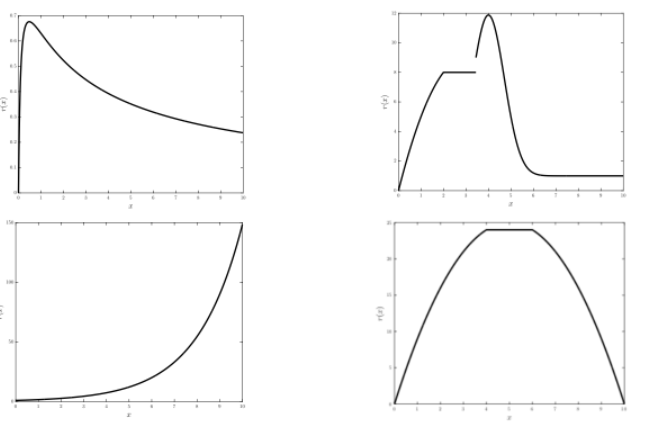
\includegraphics[width=0.8\textwidth]{Images/QuasiConcave.png}
\end{center}

\subsection{Funzioni Quasi-Convesse Differenziabili}
Facciamo alcune considerazioni:
\begin{itemize}
    \item I Punti Stazionari di una Funzione Quasi-Concava NON sono necessariamente massimi Globali e le condizioni KKT sono solo Necessarie...
    \item Una Funzione Quasi-Concava può anche non essere Differenziabile (non è neanche detto che sia continua vedendo uno dei grafici qui sopra)
    \item Una Funzione Quasi-Concava può anche essere convessa in un tratto (ad esempio guardando il primo grafico qui sopra) o totalmente (come nel terzo grafico.
\end{itemize}

\subsubsection{Condizioni al Primo Ordine}
(Senza dimostrazione)
Sia $f$ una funzione Differenziabile su un insieme $C$ Aperto e Convesso.\\
Allora $f$ è quasi-concava se e solo se:
\begin{equation*}
    f(\vc{x}_2) \leq f(\vc{x}_1) \implies \nabla(f(\vc{x}_2))^T (\vc{x}_1 - \vc{x}_2) \geq 0
\end{equation*}

\subsection{Proprietà delle Funzioni Quasi-Concave}
\subsubsection{Algebra delle Funzioni Quasi-Concave}
$f(\vc{x}) = \min\{w_1 f_1(\vc{x}),..., w_N f_N(\vc{x})\}$ è Quasi-Concava se:
\begin{itemize}
    \item $w_i \geq 0$
    \item Tutte le $f_i$ sono Quasi-Concave
\end{itemize}

Da ricordare è che la Somma di Funzioni Quasi-Concave NON è Quasi-Concava!


\section{Funzioni Pseudo-Concave}
Sia $C \subset \mathbb{R}^n$ un insieme Convesso, allora $f: C \longrightarrow \mathbb{R}$ è Pseudo-Concava se e solo se è Differenziabile e se:
\begin{equation*}
    f(\vc{x}_2) < f(\vc{x}_1) \implies \nabla(f(\vc{x}_2))^T (\vc{x}_1 - \vc{x}_2) > 0
\end{equation*}
per ogni $\vc{x}_1, \vc{x}_2 \in C$.
Viceversa $f$ si dice Strettamente Pseudo-Concava se e solo se è Differenziabile e se:
\begin{equation*}
    f(\vc{x}_2) \leq f(\vc{x}_1) \implies \nabla(f(\vc{x}_2))^T (\vc{x}_1 - \vc{x}_2) > 0
\end{equation*}
per ogni $\vc{x}_1, \vc{x}_2 \in C$.

\subsection{Punti Stazionari}
Ogni Punto Stazionario di una Funzione Pseudo-Concava è un Massimo Globale! Ed è Unico se la funzione è Strettamente Pseudo-Convava!!\\
Quindi segue che per un Problema in cui la Funzione Obiettivo è una Funzione Pseudo-Concava e con Vincoli Affini, le KKT sono Condizioni Necessarie e Sufficienti!!

\subsection{Proprietà delle Funzioni Pseudo-Concave}
\subsubsection{Concavità e Differenziabilità implica Pseudo-Concavità}
Se $f$ è concava, allora $f(\vc{x}_2) < f(\vc{x}_1)$ implica che:
\begin{equation*}
    \nabla(f(\vc{x}_2))^T (\vc{x}_1 - \vc{x}_2) > 0
\end{equation*}
\subsubsection{Ottimalità dei Punti Stazionari}
La definizione di Pseudo-Concavità possiamo invertirla così:
\begin{equation*}
    \begin{aligned}
    &\left(f(\vc{x}_2) < f(\vc{x}_1) \implies \nabla(f(\vc{x}_2))^T (\vc{x}_1 - \vc{x}_2) > 0 \right) \equiv \\ \\
    &\equiv \left(\nabla(f(\vc{x}_2))^T (\vc{x}_1 - \vc{x}_2) \leq 0 \implies f(\vc{x}_2) \geq f(\vc{x}_1) \right) 
    \end{aligned}
\end{equation*}
\\
Quindi $\vc{x}_2$ tale che $\nabla(f(\vc{x}_2)) = 0$ verifica la prima parte della relazione, quindi implica che $f(\vc{x}_2) \geq f(\vc{x}_1)$ per ogni $\vc{x}_1$.\\
\vspace{10pt}
Ma la stessa cosa NON VALE per le funzioni Quasi-Concave:\\ 
La definizione di Quasi-Concavità possiamo invertirla così:
\begin{equation*}
    \begin{aligned}
    &\left(f(\vc{x}_2) \leq f(\vc{x}_1) \implies \nabla(f(\vc{x}_2))^T (\vc{x}_1 - \vc{x}_2) \geq 0 \right) \equiv \\ \\
    &\equiv \left(\nabla(f(\vc{x}_2))^T (\vc{x}_1 - \vc{x}_2) < 0 \implies f(\vc{x}_2) > f(\vc{x}_1) \right) 
    \end{aligned}
\end{equation*}
Quindi $\vc{x}_2$ tale che $\nabla(f(\vc{x}_2)) = 0$ NON verifica la prima parte della relazione, quindi NON implica che $f(\vc{x}_2) > f(\vc{x}_1)$ per ogni $\vc{x}_1$.

\section{Concavità Generalizzata di un Rapporto}
Consideriamo il seguente rapporto:
\begin{equation*}
    R(\vc{x}) = \frac{f(\vc{x})}{g(\vc{x})}
\end{equation*}
e distinguiamo alcuni casi:
\subsection{Affine/Affine}
Supponendo $f(\vc{x}), g(\vc{x}) >0$ allora $f(\vc{x})$ è Pseudo-Concava e Pseudo-Convessa.

\subsection{Concava/Affine}
Supponendo $f(\vc{x})$ Differenziabile e Concava, e $g(\vc{x})$ affine, allora: $R(\vc{x})$ è Pseudo-Concava.

\subsection{Concava/Convessa}
Supponendo $f(\vc{x})$ Differenziabile e Concava e $g(\vc{x}) > 0$ Differenziabile e Convessa, allora $R(\vc{x})$ è Pseudo-Concava.\\ 
$R(\vc{x})$ è Quasi-Concava se cade l'ipotesi di Differenziabilità.

\subsection{Algoritmo di Dinkelbach}
Siano:
\begin{itemize}
    \item $f(\vc{x}) \geq 0$ Concava e Differenziabile
    \item $g(\vc{x}) > 0$ Convessa e Differenziabile
    \item $h_k$ Convessa per ogni k
\end{itemize}
\begin{equation*}
    \begin{cases}
    \max_{\vc{x}} \frac{f(\vc{x})}{g(\vc{x})} \\
    con \quad h_k(\vc{x}) \leq 0 \ \forall k=1,...,K
    \end{cases}
\end{equation*}
Quindi la Funzione Obiettivo è Pseudo-Concava $\implies$ le Condizioni KKT sono Necessarie e Sufficienti.\\ \\
Considerato ciò, l'algoritmo di Dinkelbach consiste nel convertire il Problema Funzionale in una sequenza di Problemi Convessi Non Frazionali.\\ 
\subsubsection{Teorema}
Consideriamo:
\begin{equation*}
    F(\lambda) = \max_{\vc{x}} \{ (f(\vc{x}) - \lambda  g(\vc{x})) \ : \ h_k(\vc{x}) \leq 0, \forall k \}
\end{equation*}
Enunciato: Esiste un unico valore $\lambda^*$ positivo, tale che $F(\lambda^*) = 0$ che risolve anche il Problema Frazionale Associato.\\
Quindi risolvere un Problema Frazionale si traduce nel trovare l'unico zero della funzione $F(\lambda)$.\\
\begin{algorithm}
\begin{algorithmic}
\Large
\State {Inizializza} $\epsilon > 0; n = 0; \lambda_n = 0;$
\Repeat
\State $\vc{x}_n^* = argmax_{\vc{x}} \{f(\vc{x} - \lambda_n g(\vc{x})) \ : \ h_k(\vc{x}) \leq 0, \forall k\};$
\State $F(\lambda_n) = f(\vc{x}_n^*) - \lambda_n g(\vc{x}_n^*);$
\State $\lambda_{n+1} = \frac{f(\vc{x}_n^*)}{g(\vc{x}_n^*)};$
\State $n = n + 1;$
\Until{$F(\lambda_n) < \epsilon$}
\end{algorithmic}
\end{algorithm}
\begin{center}
    Ciascuna iterazione rappresenta un Problema Convesso da risolvere.
\end{center}

\subsection{Esempio di Problema Convesso: Water Filling}
Consideriamo il seguente problema:
\begin{equation*}
    \begin{aligned}
    \max_{\vc{x}} \sum_{k=1}^K \log_2 (1 + c_k x_k)\\
    con \ x_k \geq 0, \forall k \\
    \sum_{k=1}^K x_k = P
    \end{aligned}
\end{equation*}
Esprimiamola in una forma più facile da utilizzare:
\begin{equation*}
    \begin{aligned}
    \min_{\vc{x}} - \sum_{k=1}^K \log_2 (1 + c_k x_k)\\
    con \ -x_k \leq 0, \forall k \\
    \sum_{k=1}^K x_k = P
    \end{aligned}
\end{equation*}
Calcoliamo il suo Lagrangiano:
\begin{equation*}
    L(\vc{x}, \vc{\lambda}, \vc{\nu}) =  - \sum_{k=1}^K \log_2 (1 + c_k x_k) - \sum_{k=1}^K \lambda_k x_k + \nu \left(\sum_{k=1}^K x_k - P \right)
\end{equation*}
Scriviamo ora le Condizioni KKT:
\begin{equation*}
    \begin{aligned}
   \underbrace{\frac{\partial L}{\partial x_n}}_{\text{Generica} \ x_n} &= \frac{-c_n/ln(2)}{1 + c_n x_n} - \lambda_n + \nu = 0 \ \forall n \\
    &-x_n \leq 0, \ \forall n \\
    &\sum_{n=1}^K x_n = P \\
    &\lambda_n \geq 0, \ \forall n \\
    &\lambda_n x_n = 0, \ \forall n
    \end{aligned}
\end{equation*}
Ora ricaviamo $\lambda_n$ dalla prima equazione:
\begin{equation*}
    \begin{aligned}
    \lambda_n &= \nu - \frac{c_n / ln(2)}{1 + c_n x_n}, \ \forall n \\
    &-x_n \leq 0, \ \forall n \\
    &\sum_{n=1}^K x_n = P \\
    &\nu - \frac{c_n / ln(2)}{1 + c_n x_n} \geq 0, \ \forall n \\
    &\left(\nu - \frac{c_n / ln(2)}{1 + c_n x_n}\right) x_n = 0, \ \forall n
    \end{aligned}
\end{equation*}
Quindi capiamo che:
\begin{itemize}
    \item Per ogni n, se $\nu \geq c_n / ln(2) \implies x_n = 0$
    \item Per ogni n, se $\nu \leq c_n / ln(2) \implies $ dall'ultima equazione ricaviamo:
\end{itemize}
\begin{equation*}
    x_n = \frac{1}{\nu ln(2)} - \frac{1}{c_n} \geq 0
\end{equation*}
Dunque possiamo scrivere:
\begin{equation*}
    x_n = max\left(0, \frac{1}{\nu ln(2)} - \frac{1}{c_n}\right)
\end{equation*}
Infine dalla terza equazione possiamo ricavare $\nu$ risolvendo questa equazione:
\begin{equation*}
    \sum_{n=1}^K max\left(0, \frac{1}{\nu ln(2)} - \frac{1}{c_n}\right) = P
\end{equation*}
\begin{center}
    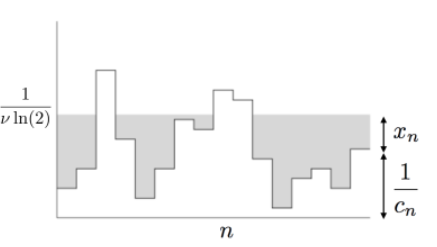
\includegraphics[width=0.8\textwidth]{Images/WaterFilling.png}
\end{center}
dove:
\begin{itemize}
    \item $1/c_n$ è il "livello del terreno"
    \item $1/\nu ln(2)$ è il "livello da raggiungere"
    \item $x_n$ è quindi la quantità di "acqua" da versare per raggiungere il livello $1/\nu ln(2)$
    \item Nel caso in cui il livello del terreno è maggiore rispetto a quello da raggiungere, "non si versa acqua" ($x_n = 0$)
\end{itemize}
\vspace{10pt}
\begin{center}
    La cosa importante è capire che più è grande $c_n$, più acqua devo versare ($x_n$).
\end{center}


\section{Problemi Multi-Obiettivo}
Ora esaminiamo il caso in cui ci siano più di una Funzione Obiettivo:
\begin{equation*}
    \begin{cases}
    \max_{\vc{x}} \{f_1(\vc{x}),...,f_N(\vc{x})\} \\
    con \quad h_i(\vc{x}) \geq 0, \forall i \\
    c_j(\vc{x}) = 0, \forall j
    \end{cases}
\end{equation*}
Questo tipo di problemi crea ambiguità sulla scelta delle soluzioni migliori dato che non esistono relazioni di ordine totale tra vettori.\\ 
Per questo motivo occorre l'utilizzo di alcune tecniche come quella di Scalarizzazione.

\subsection{Tecnica di Scalarizzazione}
Questa tecnica consiste nel convertire il problema in una forma con una Funzione Obiettivo Scalare:
\subsubsection{Somma Pesata}
Si massimizza una somma pesata delle funzioni obiettivo:
\begin{equation*}
    \begin{cases}
    \max_{\vc{x}} \sum_{n=1}^N w_n f_n(\vc{x})\\
    con \quad h_i(\vc{x}) \geq 0, \forall i\\
    c_j = 0, \forall j
    \end{cases}
\end{equation*}
con $w_n \geq$ per ogni n e tipicamente normalizzati.

\subsubsection{Minimo Pesato}
Si massimizza il Minimo Pesato delle funzioni obiettivo:
\begin{equation*}
    \begin{cases}
    \max_{\vc{x}} \min_n \{ w_n f_n(\vc{x})\}
    \\con \quad h_i(\vc{x}) \geq 0, \forall i\\
    c_j = 0, \forall j
    \end{cases}
\end{equation*}
con $w_n \geq$ per ogni n e tipicamente normalizzati.

\subsubsection{Forma Differenziabile}
Il Problema max-min qui sopra può essere riscritto nella seguente Forma Differenziabile:
\begin{equation*}
    \begin{cases}
    \max_{t, \vc{x}} t \
    con \\ h_i(\vc{x}) \geq 0, \forall i\\
    c_j = 0, \forall j \\
    w_n,f_n \geq t, \forall n
    \end{cases}
\end{equation*}
L'approccio max-min ha garanzie sul valore minimo assunto da ogni funzione obiettivo, mentre la massimizzazione di una somma pesata no.

\subsection{Frontiera di Pareto}
Diamo alcune definizioni:
\begin{itemize}
    \item Dominazione
\begin{itemize}
    \item Un vettore di funzioni $f_1^{(1)},...,f_N^{(1)}$ DOMINA un altro vettore $f_1^{(2)},...,f_N^{(2)}$ se:
\begin{equation*}
    f_n^{(1)} \geq f_n^{(2)} \ \forall n
\end{equation*}
\end{itemize}
    \item Pareto-Ottimo
    \begin{itemize}
        \item Un vettore $f_1,...,f_N$ che soddisfa i vincoli del problema si dice Pareto-Ottimo se non esiste nessun vettore $g_1,...,g_N$ che soddisfa i vincoli e tale che $f_n \leq g_n$ per ogni n
    \end{itemize}
    \item Frontiera di Pareto
    \begin{itemize}
        \item L'insieme dei vettori Pareto-Ottimi forma la Frontiera di Pareto del problema
    \end{itemize}
\end{itemize}
\begin{center}
    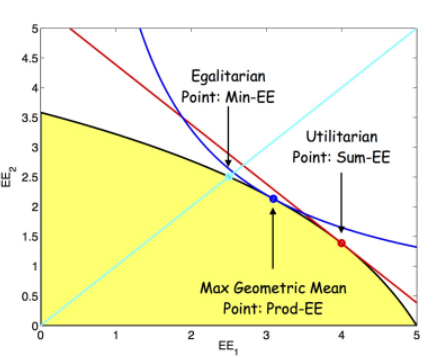
\includegraphics[width=0.8\textwidth]{Images/FrontieraPareto.png}
\end{center}